
\chapter{\propDetTitle}

In Lecture~\ref{elementarydeterminantsII} we \hyperref[detinvertible]{showed} that the determinant of a matrix is non-zero if and only if that matrix is invertible.  We also \hyperref[detmultiplicative]{showed} that the determinant is a \emph{multiplicative} function\index{Multiplicative function}, in the sense that $\det (MN)=\det M \det N$.  Now we will devise some methods for calculating the determinant.

Recall that:
\[
\det M = \sum_{\sigma} \text{sgn}(\sigma) m^1_{\sigma(1)}m^2_{\sigma(2)}\cdots m^n_{\sigma(n)}.
\]

A \emph{minor}\index{Minor} of an $n\times n$ matrix $M$ is the determinant of any square matrix obtained from $M$ by deleting one row and one column.  In particular, any entry $m^i_j$ of a square matrix~$M$ is associated to a minor obtained by deleting the $i$th row and $j$th column of~$M$.

It is possible to write the determinant of a matrix in terms of  its minors\index{Expansion by minors} as follows:

\begin{eqnarray*}
\det M &=& \sum_{\sigma} \text{sgn}(\sigma)\, m^1_{\sigma(1)}m^2_{\sigma(2)}\cdots m^n_{\sigma(n)} \\
&=& m^1_1\, \sum_{\hat{\sigma}} \text{sgn}(\hat{\sigma})\, m^2_{\hat{\sigma}(2)}\cdots m^n_{\hat{\sigma}(n)} \\
& -&  m^1_2\, \sum_{\hat{\sigma}} \text{sgn}(\hat{\sigma})\, m^2_{\hat{\sigma}(1)}m^3_{\hat{\sigma}(3)}\cdots m^n_{\hat{\sigma}(n)} \\
& +&  m^1_3\,  \sum_{\hat{\sigma}} \text{sgn}(\hat{\sigma})\, m^2_{\hat{\sigma}(1)}m^3_{\hat{\sigma}(2)}m^4_{\hat{\sigma}(4)}\cdots m^n_{\hat{\sigma}(n)} \pm \cdots
\end{eqnarray*}
Here the symbols $\hat{\sigma}$ refer to permutations of $n-1$ objects.  What we're doing here is collecting up all of the terms of the original sum that contain the first row entry $m^1_j$ for each column number $j$.  Each term in that collection is associated to a permutation sending $1\rightarrow j$.  The remainder of any such permutation maps the set $\{2, \ldots, n \}\rightarrow \{1, \ldots, j-1, j+1, \ldots, n \}$.  We call this partial permutation $\hat{\sigma}=\begin{bmatrix} \sigma(2) & \cdots & \sigma(n) \end{bmatrix}$.

The last issue is that the permutation $\hat{\sigma}$ may not have the same sign as $\sigma$.  From previous homework, we know that a permutation has the same parity as its inversion number.  Removing $1\rightarrow j$ from a permutation  reduces the inversion number by the number of elements right of $j$ that are less than~$j$.  Since $j$ comes first in the permutation $\begin{bmatrix}j & \sigma(2) & \cdots & \sigma(n) \end{bmatrix}$, the inversion number of $\hat{\sigma}$ is reduced by $j-1$.  Then the sign of~$\sigma$ differs from the sign of~$\hat{\sigma}$ if $\sigma$ sends $1$ to an even number.

In other words, to expand by minors we pick an entry $m^1_j$ of the first row, then add $(-1)^{j-1}$ times the determinant of the matrix with row $i$ and column~$j$ deleted.

\begin{example}
Let's compute the determinant of 
$M=\begin{pmatrix}
1 & 2 & 3 \\
4 & 5 & 6 \\
7 & 8 & 9 \\
\end{pmatrix}$ using expansion by minors.

\begin{eqnarray*}
\det M & = & 1\det \begin{pmatrix}
5 & 6 \\
8 & 9 \\
\end{pmatrix}
-2 \det \begin{pmatrix}
4 & 6 \\
7 & 9 \\
\end{pmatrix}
+3 \det \begin{pmatrix}
4 & 5 \\
7 & 8 \\
\end{pmatrix} \\
& = & 1(5\cdot 9- 8\cdot 6) -2 (4\cdot 9- 7\cdot 6) + 3 (4\cdot 8- 7\cdot 5) \\
& = & 0 \\
\end{eqnarray*}
Here, $M^{-1}$ does not exist because\footnote{A fun exercise is to compute the determinant of a $4\times 4$ matrix filled in order, from left to right,  with the numbers $1,2,3,\ldots 16$. What do you observe? Try the same for a $5\times 5$ matrix with $1,2,3\ldots 25$. Is there a pattern? Can you explain it?} $\det M=0.$
\end{example}


\begin{example}
Sometimes the entries of a matrix allow us to simplify the calculation of the determinant.  Take $N= \begin{pmatrix}
1 & 2 & 3 \\
4 & 0 & 0 \\
7 & 8 & 9 \\
\end{pmatrix}$.  Notice that the second row has many zeros; then we can switch the first and second rows of $N$ to get:

\begin{eqnarray*}
\det \begin{pmatrix}
1 & 2 & 3 \\
4 & 0 & 0 \\
7 & 8 & 9 \\
\end{pmatrix} & = & -\det \begin{pmatrix}
4 & 0 & 0 \\
1 & 2 & 3 \\
7 & 8 & 9 \\
\end{pmatrix}\\
&=& -4 \det \begin{pmatrix}
2 & 3 \\
8 & 9 \\
\end{pmatrix} \\
&=& 24
\end{eqnarray*}
\end{example}
 
\videoscriptlink{properties_of_determinant_practice.mp4}{Example}{video_properties_of_determinant_practice}

\begin{theorem}
For any square matrix $M$, we have:
\[
\det M^T = \det M
\]
\end{theorem}
\begin{proof}
  By definition, \[
\det M = \sum_{\sigma} \text{sgn}(\sigma) m^1_{\sigma(1)}m^2_{\sigma(2)}\cdots m^n_{\sigma(n)}.
\]

For any permutation $\sigma$, there is a unique inverse permutation $\sigma^{-1}$ that undoes $\sigma$.  If $\sigma$ sends $i\rightarrow j$, then $\sigma^{-1}$ sends $j\rightarrow i$.  In the two-line notation for a permutation, this corresponds to just flipping the permutation over.  For example, if $\sigma=\begin{bmatrix} 
1 & 2 & 3 \\
2 & 3 & 1
\end{bmatrix}$, then we can find $\sigma^{-1}$ by flipping the permutation and then putting the columns in order:

\[
\sigma^{-1}=\begin{bmatrix} 
2 & 3 & 1 \\
1 & 2 & 3
\end{bmatrix}=\begin{bmatrix} 
1 & 2 & 3 \\
3 & 1 & 2
\end{bmatrix}
\]
Since any permutation can be built up by transpositions, one can also find the inverse of a permutation $\sigma$ by undoing each of the transpositions used to build up $\sigma$; this shows that one can use the same number of transpositions to build $\sigma$ and $\sigma^{-1}$.  In particular, $\sgn \sigma= \sgn \sigma^{-1}$.

%\begin{center}\href{\webworkurl ReadingHomework14/1/}{Reading homework: problem 14.1}\end{center}
\reading{14}{1}

Then we can write out the above in formulas as follows:
\begin{eqnarray*}
\det M &=& \sum_{\sigma} \text{sgn}(\sigma) m^1_{\sigma(1)}m^2_{\sigma(2)}\cdots m^n_{\sigma(n)} \\
&=& \sum_{\sigma} \text{sgn}(\sigma) m_1^{\sigma^{-1}(1)}m_2^{\sigma^{-1}(2)}\cdots m_n^{\sigma^{-1}(n)} \\
&=& \sum_{\sigma} \text{sgn}(\sigma^{-1}) m_1^{\sigma^{-1}(1)}m_2^{\sigma^{-1}(2)}\cdots m_n^{\sigma^{-1}(n)} \\
&=& \sum_{\sigma} \text{sgn}(\sigma) m_1^{\sigma(1)}m_2^{\sigma(2)}\cdots m_n^{\sigma(n)} \\
&=& \det M^T.
\end{eqnarray*}
The second-to-last equality is due to the existence of a unique inverse permutation: summing over permutations is the same as summing over all inverses of permutations.  The final equality is by the definition of the transpose.
\end{proof}

\begin{center}

\includegraphics[scale=.25]{\propDetPath/detMT.jpg}
\end{center}

\begin{example}
Because of this theorem, we see that expansion by minors also works over columns.  Let $M=\begin{pmatrix}
1 & 2 & 3 \\
0 & 5 & 6 \\
0 & 8 & 9 \\
\end{pmatrix}$.  Then \[\det M = \det M^T = 1\det \begin{pmatrix}
5 & 8 \\
6 & 9 \\
\end{pmatrix}=-3\, .\]
\end{example}

\section{Determinant of the Inverse}

Let $M$ and $N$ be $n\times n$ matrices.
We previously showed that 

\[
\det (MN)=\det M \det N \text{, and } \det I=1.
\]
Then $1 = \det I = \det (MM^{-1}) = \det M \det M^{-1}$.  As such we have:
\begin{theorem}
\[
\det M^{-1} = \frac{1}{\det M}
\]
\end{theorem}

Just so you don't forget this:
\begin{center}

\includegraphics[scale=.3]{\propDetPath/detMm1.jpg}
\end{center}


\section{Adjoint of a Matrix}


Recall that for the $2\times 2$ matrix 
%\begin{figure}
\begin{center}
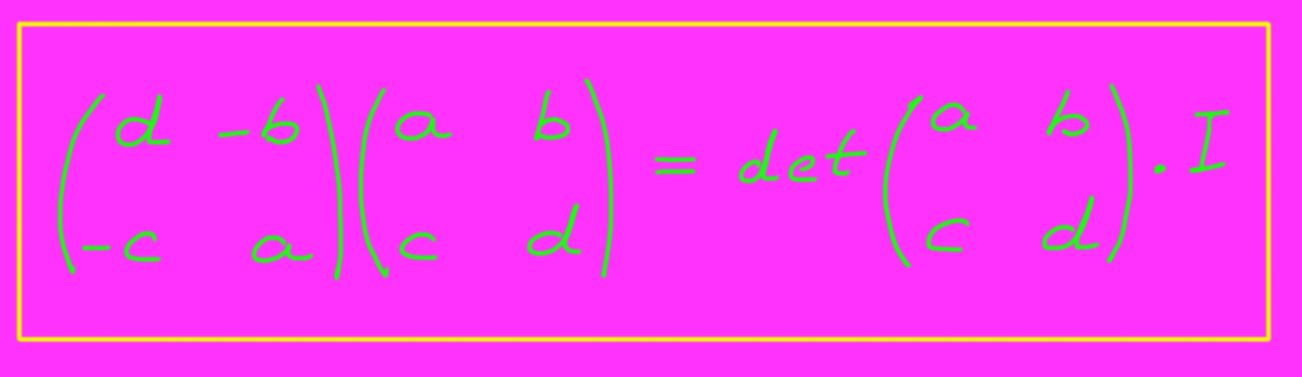
\includegraphics[scale=.2]{\propDetPath/adj2x2.jpg}
\end{center}
%\end{figure}
Or in a more careful notation: if
$M=\begin{pmatrix}
m^1_1 & m^1_2 \\
m^2_1 & m^2_2 \\
\end{pmatrix}$, then \[M^{-1}=\frac{1}{m^1_1m^2_2-m^1_2m^2_1}\begin{pmatrix}
m^2_2 & -m^1_2 \\
-m^2_1 & m^1_1 \\
\end{pmatrix}\, ,\]
so long as $\det M=m^1_1m^2_2-m^1_2m^2_1\neq 0$.
  The  matrix $\begin{pmatrix}
m^2_2 & -m^1_2 \\
-m^2_1 & m^1_1 \\
\end{pmatrix}$ that appears above is a special matrix, called the \emph{adjoint} of $M$.  Let's define the adjoint for an $n \times n$ matrix.


The \emph{cofactor}\index{Cofactor} of $M$ corresponding to the entry $m^i_j$ of $M$ 
%and then deleting the $i$th row and $j$th column of $M$, taking the determinant of the 
is the prooduct of the minor associated to $m^i_j$
%resulting matrix, and 
%multiplying by
times $(-1)^{i+j}$.  This is written $\cofactor(m^i_j)$.

\begin{definition}
For $M=(m^i_j)$ a square matrix, The \emph{adjoint matrix} $\adj M$ is given by:
\[
\adj M = (\cofactor(m^i_j))^T
\]
\end{definition}

\begin{example}
\[
\adj \begin{pmatrix}
3 & -1 & -1 \\
1 & 2 & 0 \\
0 & 1 & 1 \\
\end{pmatrix}
=
\begin{pmatrix}
\det \begin{pmatrix}
2 & 0 \\
1 & 1 
\end{pmatrix}
& -\det \begin{pmatrix}
1 & 0 \\
0 & 1 
\end{pmatrix}
& \det \begin{pmatrix}
1 & 2 \\
0 & 1 
\end{pmatrix}
\\
-\det \begin{pmatrix}
-1 & -1 \\
1 & 1 
\end{pmatrix}
& \det \begin{pmatrix}
3 & -1 \\
0 & 1 
\end{pmatrix}
& -\det \begin{pmatrix}
3 & -1 \\
0 & 1 
\end{pmatrix}
\\
\det \begin{pmatrix}
-1 & -1 \\
2 & 0 
\end{pmatrix}
& -\det \begin{pmatrix}
3 & -1 \\
1 & 0 
\end{pmatrix}
& \det \begin{pmatrix}
3 & -1 \\
1 & 2 
\end{pmatrix}
\\
\end{pmatrix}^T
\]
\end{example}

%\begin{center}\href{\webworkurl ReadingHomework14/2/}{Reading homework: problem 14.2}\end{center}
\reading{14}{2}

Let's multiply $M\adj M$.  For any matrix $N$, the $i, j$ entry of $MN$ is given by taking the dot product of the $i$th row of $M$ and the $j$th column of $N$.  
Notice that the dot product of the $i$th row of $M$ and the $i$th column of $\adj M$ is just the expansion by minors of $\det M$ in the $i$th row.
Further, notice that the dot product of the $i$th row of $M$ and the $j$th column of $\adj M$ with $j\neq i$ is the same as expanding $M$ by minors, but with the $j$th row replaced by the $i$th row.  Since the determinant of any matrix with a row repeated is zero, then these dot products are zero as well.

We know that the $i,j$ entry of the product of two matrices is the dot product of the $i$th row of the first by the $j$th column of the second.  Then:
\[
M\adj M = (\det M) I
\]

Thus, when $\det M\neq 0$, the adjoint gives an explicit formula for $M^{-1}$.


\begin{theorem}
For $M$ a square matrix with $\det M\neq 0$ (equivalently, if $M$ is invertible), then
\[
M^{-1}=\frac{1}{\det M}\adj M
\]
\end{theorem}

\videoscriptlink{properties_of_determinant_adjoint.mp4}{The Adjoint Matrix}{video_properties_of_determinant_adjoint}


\begin{figure}
\begin{center}

\includegraphics[scale=.3]{\propDetPath/adjM.jpg}
\end{center}
\end{figure}

\begin{example}
Continuing with the previous example,
\[
\adj \begin{pmatrix}
3 & -1 & -1 \\
1 & 2 & 0 \\
0 & 1 & 1 \\
\end{pmatrix} = \begin{pmatrix}
2 & 0 & 2 \\
-1 & 3 & -1 \\
1 & -3 & 7 \\
\end{pmatrix}.
\]

Now, multiply:

\begin{eqnarray*}
\begin{pmatrix}
3 & -1 & -1 \\
1 & 2 & 0 \\
0 & 1 & 1 \\
\end{pmatrix}
\begin{pmatrix}
2 & 0 & 2 \\
-1 & 3 & -1 \\
1 & -3 & 7 \\
\end{pmatrix}
&=&
\begin{pmatrix}
6 & 0 & 0 \\
0 & 6 & 0 \\
0 & 0 & 6 \\
\end{pmatrix} \\[1mm]
\Rightarrow \begin{pmatrix}
3 & -1 & -1 \\
1 & 2 & 0 \\
0 & 1 & 1 \\
\end{pmatrix}^{-1} & = & \frac{1}{6}\begin{pmatrix}
2 & 0 & 2 \\
-1 & 3 & -1 \\
1 & -3 & 7 \\
\end{pmatrix}
\end{eqnarray*}

This process for finding the inverse matrix is sometimes called \emph{Cramer's~Rule}~\index{Cramer's rule}.
\end{example}

\section{Application: Volume of a Parallelepiped}

Given three vectors $u,v,w$ in $\Re^3$, the parallelepiped\index{Parallelepiped} determined by the three vectors is the ``squished'' box whose edges are parallel to $u, v$, and $w$ as depicted in Figure~\ref{parallelepiped}.

From calculus, we know that the volume of this object is $|u\dotprod (v\times w)|$.  This is the same as expansion by minors of the matrix whose columns are $u,v,w$.  Then:
\[
\text{Volume}=\big|\det \begin{pmatrix}u & v & w \end{pmatrix} \big|
\] 



\begin{figure}
\begin{center}
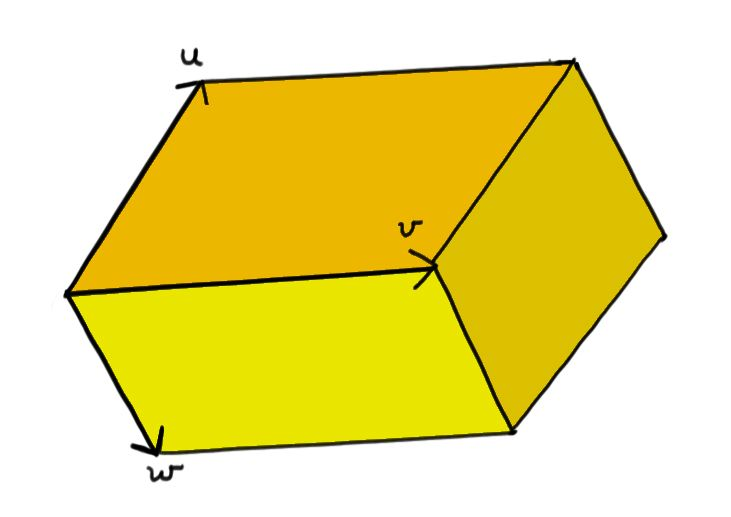
\includegraphics[scale=.4]{parallelepiped.jpg}
\caption{A parallelepiped.\label{parallelepiped}}
\end{center}
\end{figure}



%\section*{References}
%Hefferon, Chapter Four, Section I.1 and I.3
%\\
%Beezer, Chapter D, Section DM, Subsection DD
%\\
%Beezer, Chapter D, Section DM, Subsection CD
%\\
%Wikipedia:
%\begin{itemize}
%\item \href{http://en.wikipedia.org/wiki/Determinant}{Determinant}
%\item \href{http://en.wikipedia.org/wiki/Elementary_matrix}{Elementary Matrix}
%\item \href{http://en.wikipedia.org/wiki/Cramers_rule}{Cramer's Rule}
%\end{itemize}




\section{Review Problems}




\begin{enumerate}
\item \label{det33} Let $M=\begin{pmatrix}
m^1_1 & m^1_2 & m^1_3\\
m^2_1 & m^2_2 & m^2_3\\
m^3_1 & m^3_2 & m^3_3\\
\end{pmatrix}$.  Use row operations to put $M$ into \emph{row echelon form}.  For simplicity, assume that $m_1^1\neq 0 \neq m^1_1m^2_2-m^2_1m^1_2$.

Prove that $M$ is non-singular if and only if:
\[
m^1_1m^2_2m^3_3 
- m^1_1m^2_3m^3_2 
+ m^1_2m^2_3m^3_1 
- m^1_2m^2_1m^3_3 
+ m^1_3m^2_1m^3_2
- m^1_3m^2_2m^3_1
\neq 0
\]

\phantomnewpage

\item 
\begin{enumerate}
\item What does the matrix $E^1_2=\begin{pmatrix}
0 & 1 \\
1 & 0
\end{pmatrix}$ do to $M=\begin{pmatrix}
a & b \\
d & c
\end{pmatrix}$ under left multiplication?  What about right multiplication?
\item Find elementary matrices $R^1(\lambda)$ and $R^2(\lambda)$ that respectively multiply rows $1$ and $2$ of $M$ by $\lambda$ but otherwise leave $M$ the same under left multiplication.
\item Find a matrix $S^1_2(\lambda)$ that adds a multiple $\lambda$ of row $2$ to row $1$ under left multiplication.
\end{enumerate}

\phantomnewpage

\item Let $M$ be a matrix and $S^i_jM$ the same matrix with rows \(i\) and \(j\) switched.  Explain every line of the 
\hyperlink{rowswap}{series of equations} proving that $\det M = -\det (S^i_jM)$.

\phantomnewpage

%\item \label{prob_inversion_number} This problem is a ``hands-on'' look at why \hyperlink{permutation_parity}{the property} describing the parity of permutations is true.
%
%\hypertarget{inversion_number}{The \emph{inversion number}}\index{Permutation!Inversion number} of a permutation $\sigma$ is the number of pairs $i<j$ such that $\sigma(i)>\sigma(j)$; it's the number of ``numbers that appear left of smaller numbers'' in the permutation.  For example, for the permutation $\rho = [4,2,3,1]$, the inversion number is $5$. The number $4$ comes before $2,3,$ and $1$, and $2$ and $3$ both come before $1$.
%
%Given a permutation $\sigma$, we can make a new permutation $\tau_{i,j} \sigma$ by exchanging the $i$th and $j$th entries of $\sigma$.
%
%\begin{enumerate}
%\item What is the inversion number of the permutation \(\mu=[1,2,4,3]\) that exchanges 4 and 3 and leaves everything else alone? Is it an even or an odd permutation?
%
%\item What is the inversion number of the permutation \(\rho=[4,2,3,1]\) that exchanges 1 and 4 and leaves everything else alone? Is it an even or an odd permutation?
%
%\item What is the inversion number of the permutation \(\tau_{1,3} \mu\)? Compare the parity\footnote{The \emph{parity} of an integer refers to whether the integer is even or odd. Here the parity of a permutation $\mu$ refers to the parity of its inversion number.} of \(\mu\) to the parity of \(\tau_{1,3} \mu.\)
%
%\item What is the inversion number of the permutation \(\tau_{2,4} \rho\)? Compare the parity of \(\rho\) to the parity of \(\tau_{2,4} \rho.\)
%
%\item What is the inversion number of the permutation \(\tau_{3,4} \rho\)? Compare the parity of \(\rho\) to the parity of \(\tau_{3,4} \rho.\)
%\end{enumerate}
%
%\videoscriptlink{elementary_matrices_determinant_hint.mp4}{Problem~\ref{prob_inversion_number} hints}{scripts_elementary_matrices_determinants_hint}

\phantomnewpage

%\item \label{problem_permutation} (Extra credit) Here we will examine a (very) small set of the general properties about permutations and their applications. In particular, we will show that one way to compute the sign of a permutation is by finding the \hyperlink{inversion_number}{inversion number} $N$ of $\sigma$ and we have
%\[
%\sgn(\sigma) = (-1)^N.
%\]
%
%For this problem, let $\mu = [1,2,4,3]$.
%
%\begin{enumerate}
%\item Show that every permutation $\sigma$ can be sorted by only taking simple (adjacent) transpositions\index{Permutation!Simple transposition} $s_i$ where $s_i$ interchanges the numbers in position $i$ and $i+1$ of a permutation $\sigma$ (in our other notation $s_i = \tau_{i,i+1}$). For example $s_2 \mu = [1, 4, 2, 3]$, and to sort $\mu$ we have $s_3 \mu = [1, 2, 3, 4]$.
%
%\item \label{prob_part_relations} We can compose simple transpositions together to represent a permutation (note that the sequence of compositions is not unique), and these are associative, we have an identity (the trivial permutation where the list is in order or we do nothing on our list), and we have an inverse since it is clear that $s_i s_i \sigma = \sigma$. Thus permutations of $[n]$ under composition are an example of a \hyperref[groups]{group}. However note that not all simple transpositions commute with each other since
%\begin{align*}
%s_1 s_2 [1, 2, 3] & = s_1 [1, 3, 2] = [3, 1, 2]
%\\ s_2 s_1 [1, 2, 3] & = s_2 [2, 1, 3] = [2, 3, 1]
%\end{align*}
%(you will prove here when simple transpositions commute). When we consider our initial permutation to be the trivial permutation $e = [1, 2, \dotsc, n]$, we do not write it; for example $s_i \equiv s_i e$ and $\mu = s_3 \equiv s_3 e$. This is analogous to not writing 1 when multiplying. Show that $s_i s_i = e$ (in shorthand $s_i^2 = e$), $s_{i+1} s_i s_{i+1} = s_i s_{i+1} s_i$ for all $i$, and $s_i$ and $s_j$ commute for all $|i - j| \geq 2$.
%
%\item Show that every way of expressing $\sigma$ can be obtained from using the relations proved in part~\ref{prob_part_relations}. In other words, show that for any expression $w$ of simple transpositions representing the trivial permutation $e$, using the proved relations.
%
%\emph{Hint: Use induction on $n$. For the induction step, follow the path of the $(n+1)$-th strand by looking at $s_n s_{n-1} \cdots s_k s_{k\pm1} \cdots s_n$ and argue why you can write this as a subexpression for any expression of $e$. Consider using diagrams of these paths to help.}
%
%\item The simple transpositions \hyperlink{action}{acts on} an $n$-dimensional vector space $V$ by $s_i v = E^i_{i+1} v$ (where $E^i_j$ is \hyperlink{elem_matrix_row_swap}{an elementary matrix}) for all vectors $v \in V$. Therefore we can just represent a permutation $\sigma$ as the matrix $M_{\sigma}$\footnote{Often people will just use $\sigma$ for the matrix when the context is clear.}, and we have $\det(M_{s_i}) = \det(E^i_{i+1}) = -1$. Thus prove that $\det(M_{\sigma}) = (-1)^N$ where $N$ is a number of simple transpositions needed to represent $\sigma$ as a permutation. You can assume that $M_{s_i s_j} = M_{s_i} M_{s_j}$ (it is not hard to prove) and that $\det(A B) = \det(A) \det(B)$ \hyperref[detmultiplicative]{from Chapter~\ref*{elementarydeterminantsII}}.
%
%\emph{Hint: You to make sure $\det(M_{\sigma})$ is well-defined since there are infinite ways to represent $\sigma$ as simple transpositions.}
%
%\item Show that $s_{i+1} s_i s_{i+1} = \tau_{i, i+2}$, and so give one way of writing $\tau_{i, j}$ in terms of simple transpositions? Is $\tau_{i,j}$ an even or an odd permutation? What is $\det(M_{\tau_{i,j}})$? What is the inversion number of $\tau_{i,j}$?
%
%\item The minimal number of simple transpositions needed to express $\sigma$ is called the \emph{length}\index{Permutation!Length} of $\sigma$; for example the length of $\mu$ is 1 since $\mu = s_3$. Show that the length of $\sigma$ is equal to the inversion number of $\sigma$.
%
%\emph{Hint: Find an procedure which gives you a new permutation $\sigma^{\prime}$ where $\sigma = s_i \sigma^{\prime}$ for some $i$ and the inversion number for $\sigma^{\prime}$ is 1 less than the inversion number for $\sigma$.}
%
%\item Show that $(-1)^N = \sgn(\sigma) = \det(M_{\sigma})$, where $\sigma$ is a permutation with $N$ inversions. Note that this immediately implies that $\sgn(\sigma \rho) = \sgn(\sigma) \sgn(\rho)$ for any permutations $\sigma$ and $\rho$.
%\end{enumerate}

\item Let $M'$ be the matrix obtained from $M$ by swapping two columns $i$ and $j$. Show that $\det M'=-\det M $.

\item The scalar triple product of three vectors $u,v,w$ from $\Re^3$ is $u\cdot(v\times w)$. Show that this product is the same as the determinant of the matrix whose columns are $u,v,w$ (in that order). What happens to the scalar triple product when the factors are permuted? 

\item Show that if $M$ is a $3\times 3$ matrix whose third row is a sum of multiples of the other rows ($R_3=aR_2+bR_1$) then $\det M=0$. Show that the same is true if one of the columns is a sum of multiples of the others. 

\end{enumerate}

\phantomnewpage

\newpage




